\documentclass[times, utf8, diplomski]{fer}
\usepackage{booktabs}
\usepackage[utf8]{inputenc}

\usepackage[T1]{fontenc}
\usepackage{fixltx2e}
\usepackage{graphicx}
\usepackage{longtable}
\usepackage{float}
\usepackage{wrapfig}
\usepackage{soul}
\usepackage{textcomp}
\usepackage{marvosym}
\usepackage{wasysym}
\usepackage{latexsym}
\usepackage{amssymb}
\usepackage{hyperref}
\usepackage{caption}
\usepackage{pdfpages}
\usepackage{float}
%\usepackage[usenames, dvipsnames]{color}
\usepackage{listings}
\usepackage{xcolor}
\usepackage{subfig}
\usepackage{algpseudocode}
\usepackage[Algoritam]{algorithm}
\usepackage{amssymb}

\lstset { %
    language=C++,
    backgroundcolor=\color{black!5}, % set backgroundcolor
    basicstyle=\footnotesize,% basic font setting
}


\begin{document}

\thesisnumber{570}

\title{Tool for aligning long DNA reads}

\author{Filip Paveti\'{c}}

\maketitle

% Ispis stranice s napomenom o umetanju izvornika rada. Uklonite naredbu \izvornik ako želite izbaciti tu stranicu.
\izvornik

% Dodavanje zahvale ili prazne stranice. Ako ne želite dodati zahvalu, naredbu ostavite radi prazne stranice.
\zahvala{\\
Zahvaljujem Mili Šikiću na zadatku, strpljenju i diskusijama.\\
\\
Hvala roditeljima za sve. Bez vas mnogo toga bi bilo mnogo teže.}

\tableofcontents

\chapter{Introduction}

Through the past few years, DNA sequencing methods have advanced significantly. Massively parallel sequencing methods have become very common in biological research, resulting in very broad applications, for example in infectious disease or cancer research. Due to decreasing cost and increasing usage large ammounts of data are gathered through various experiments.\\
\\
Resequencing a human genome cost several billion dollars at the turn of the millennium, reduced to \$10,000 at the start of 2011. By year's end, the equivalent genome is projected to cost only \$2,000\cite{SNAP}. This is a consequence of intensive labor and research done by scientists all over the world. All the parts in the genome analyzing pipeline are advancing fast. Popular analysis of the human genome consists of reading the DNA pieces - \emph{reads} - of a person with a sequencing machine and comparing the reads with the reference human genome which has been previously reliably assembled. This is a computationally very intensive task. Currently, most popular sequencing machines produce reads of length up to several thousands and many algorithms have been developed to handle this kind of data. However, sequencing methods are improving their speed, read length and accuracy. With the increasing length of the read on the output of the sequencing machines there is a need for new algorithms which could manage the new data. This Thesis addresses that need and gives some ideas on what to do. Alignment tool named LISA is developed which implements the novel concepts discussed throughout the Thesis.\\
\\
Chapter 2 gives an introductory tutorial to genetics and bioinformatics algorithms.\\
Chapter 3 gives descriptions of the concepts used in LISA and implementation details.\\
Chapter 4 contains results of the simulations and comparison with some of the existing aligners.

\chapter{Preliminaries}

From algorithmic point of view, aligning reads to a reference genome comes down to string pattern matching. When looked that way, one does not have to know a lot of biology background in order to understand how the existing alignment systems work. However, to understand a wider picture it is useful to know some basic genetics. 
\\
\\
This chapter is intended to give a short introduction to genetics. There exist many resources which cover this topic in far more depth\cite{griffiths}\cite{brown}. Additionaly, terminology used through rest of the Thesis is introduced. In the end of the chapter, basic alignment algorithms are discussed in details.

\section{Genetics}
\subsection{Overview}

\emph{Genetics} is a field of science which studies \emph{genes}. Genes are the carrier of biological information in the living organisms. They are responsible for inheritance of features from organisms to their offsprings. Aside from carrying that hereditary information, the role of genes inside a cell of an organism is to dictate production of molecules called \emph{proteins}. If we think of a gene as a part of the cell which commands what to do, protein is the part which does the job. Each type of protein is specialized for a particular job, such as catalyzing metabolic reactions, replicating  DNA or transporting molecules from one place to another.
\\
\\
Protein is structured as a chain of twenty different kinds of molecules called \emph{amino-acids}. Interaction between those molecules causes the protein to fold into a compact shape (Figure \ref{myoglobin}). Shape and sequence of amino-acids\footnote{Amino-acids in the chain are called residues.} determine what a protein does. For example, protein can match the shape of another molecule, which would allow the protein to bind around that molecule and transport it.

\begin{figure}[!ht]
\begin{center}
	\includegraphics[width=0.7\textwidth]{../img/Myoglobin.png}
	\caption{3D structure of Myoglobin protein\protect\cite{myoglobin.img}}\label{myoglobin}
\end{center}
\end{figure}

\subsection{From genes to proteins}

\emph{DNA (deoxyribonucleid acid)} is a long molecule which encodes genetic instructions in living organisms. That molecule consists of two interconnected chains (\emph{strands}) which are consisted of alternating sugar and phosphate groups with one of four kind of \emph{nucleobases} attached to the sugars. Nucleobases found in the DNA are: guanine, adenine, thymine and cytosine encoded using letters G, A, T and C respectively. Bases on the two strands are always paired: next to adenine on one strand there is always thymine on the other. Opposite to guanine there is always cytosine. Due to their chemical composition, strands have directionality. Ends of strands are denoted by 5' and 3'. Those numbers refer to the orientation of fifth and third carbon atom sugar molecules are facing. Many processes involving DNA are directed (for example, replication occurs only in 5'-3' direction). Total DNA of an organism is packed inside of one or more structures called \emph{chromosomes}. Genes are only special segments of DNA which encode instruction for protein production. Set of all genes in an organism is called the \emph{genome}.
\\

\begin{figure}[!ht]
\begin{center}
	\includegraphics[width=0.5\textwidth]{../img/DNA_chemical_structure.pdf}
	\caption{DNA chemical structure\protect\cite{dna.chemical.structure.img}}\label{dna.chemical.structure}
\end{center}
\end{figure}

Process of protein production contains several steps. First, cell reads a gene and \emph{transcribes} it into \emph{RNA} chain. That molecule either has a function on its own or is passed to a structure called \emph{ribosome} - its role is to \emph{translate} received RNA to a protein.
\\

\begin{figure}[!ht]
\begin{center}
	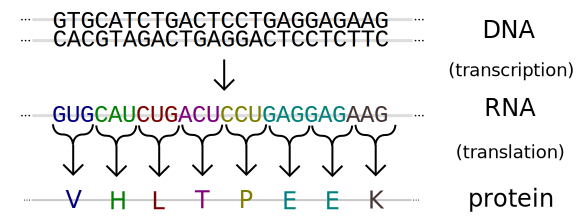
\includegraphics[width=0.7\textwidth]{../img/Genetic_code.pdf}
	\caption{DNA transcription and translation\cite{dna.transcription.translation.img}}\label{genetic.code}
\end{center}
\end{figure}

Transcription step is conceptually straight forward - one of the strands of DNA is copied replacing every thymine (T) occurence with uracil (U), creating the RNA chain. Finally in the translation step RNA is passed to a ribosome. It translates consecutive triplets of bases into corresponding amino-acids resulting in a protein. 

\section{Shotgun DNA sequencing}

Shotgun sequencing is a method of determining the order of nucleotides in a DNA strand. Current technologies allow efficients sequencing of fairly short strands (100 to 1000 basepairs). That is why a long strand is copied several times and each clone broken at random places into \emph{fragments}. This process inspired the name of the method since it imitates random firing pattern of an actual shotgun. Due to loss of precision not entire fragments are actually read. In the case of \emph{single} end sequencing some number of bases from one end of the fragment is read whereas in the case of \emph{paired} end sequencing both ends are read simultaneously, keeping track of distance between them and their orientation. After DNA reads of an organism have been accumulated\footnote{One accepted way is to produce one or two files in the FASTQ format, depending on whether it is a single or paired end sequencing involved.}, DNA is then assembled with the help of computers. 

\begin{figure}[!ht]
\begin{center}
	\includegraphics[width=0.85\textwidth]{../img/Whole_genome_shotgun_sequencing.png}
	\caption{Whole genome shotgun sequencing\cite{shotgun.sequencing.img}}\label{shotgun.sequencing}
\end{center}
\end{figure}

\section{Alignment algorithms}

One of the fundamental problems of finding good overlap between reads or aligning them to a reference genome is that the matchings we are looking for need not to be perfect. This is a consequence of errors which are introduced to the reads, either by the sequencing process or by mutations. In order to deal with that, algorithms such as Smith-Waterman\cite{Smith1981195}, Needleman-Wunsch\cite{nw}  and Levenshtein distance\cite{edit.distance.tutorial} have been developed. In the succeeding section algorithm for calculating the Levenshtein distance is described. The section will introduce the basic concept on top of the other mentioned algorithms are built as well.

\subsection{Edit (Levenshtein) distance}
\label{edit.distance.algo}

Levenshtein or edit distance is a metric measuring the difference between two sequences. Simply stated, it is a minimum number of single character edits (insertions, deletions and substitutions) required to change one word into the other.
\\
\\
Mathematically, edit distance of strings $a$ and $b$ is given by $d_{a,b}(|a|,|b|)$ where:

\begin{eqnarray}
	\label{levenshtein}
	d_{a,b}\left(i,j\right) & = & 
							\left\{
								\begin{array}{ll}
								max(i,j) & \mbox{if } min(i,j) = 0\\	
								min\left\{
									\begin{array}{ll}
									d_{a,b}(i-1,j)\\	
									d_{a,b}(i,j-1)\\	
									d_{a,b}(i-1,j-1) + [a_i\ne b_i]\\	
									\end{array}
									\right.&\mbox{otherwise}\\
								\end{array}
							\right.
\end{eqnarray}

\subsubsection{Example}
Levenhstein distance between words "kitten" and "sitting" is 3, with the following sequence of operations:

\begin{enumerate}\itemsep0pt
\item \textbf{k}itten $\rightarrow$ \textbf{s}itten (substitution)
\item sitt\textbf{e}n $\rightarrow$ sitt\textbf{i}n (substitution)
\item sittin $\rightarrow$ sittin\textbf{g} (insertion)
\end{enumerate}
The simplest way to do the calculation is to fill out a table like this:

\begin{table}[H]
\centering
\small
\begin{tabular}{|c|c|c|c|c|c|c|c|}
\hline
	   &   & \textbf{k} & \textbf{i} & \textbf{t} & \textbf{t} & \textbf{e} & \textbf{n}\\
\hline
	   & 0 & 1 & 2 & 3 & 4 & 5 & 6\\
\hline
	 \textbf{s} & 1 & 1 & 2 & 3 & 4 & 5 & 6\\
\hline
	 \textbf{i} & 2 & 2 & 1 & 2 & 3 & 4 & 5\\
\hline
	 \textbf{t} & 3 & 3 & 2 & 1 & 2 & 3 & 4\\
\hline
	 \textbf{t} & 4 & 4 & 3 & 2 & 1 & 2 & 3\\
\hline
	 \textbf{i} & 5 & 5 & 4 & 3 & 2 & 2 & 3\\
\hline
	 \textbf{n} & 6 & 6 & 5 & 4 & 3 & 3 & 2\\
\hline
	 \textbf{g} & 7 & 7 & 6 & 5 & 4 & 4 & 3\\
\hline

\end{tabular}
\caption{Calculating Levenshtein distance between "kitten" and "sitting"}\label{levenshtein.table}
\end{table}

\subsubsection{Complexity}
Direct implementation of the above calculation is proportional with lengths of both input string. More precisely, there are $O(|a||b|)$ operations needed (and the same ammount of memory). If assumption that a distance between $a$ and $b$ does not exceed $k$ is fullfilled, it is enough only to fill diagonal stripe of width $2k+1$ in the matrix. Using that observation complexity is reduced to $O(k*min(|a|,|b|))$. In practice, this implementation is shown to be very usefull (for example, SNAP\cite{SNAP})


\chapter{LISA - Longest Increasing Subsequence Aligner}
\section{Overview}
This chapter begins by an overview of the algorithms used by modern mappers. After that, approach developed in this Thesis is described in details.\\
\\
One of the first algorithms developed for aligning reads is a \emph{local alignment} algorithm called Smith-Waterman\cite{Smith1981195}. Alignments received by that algorithm are considered very accurate. Unfortunately, its time-complexity\footnote{This is briefly discussed in chapter 2.} limits the usage practicality so more advanced algorithms have been developed through the years.\\
\\
Many modern mappers (such as SNAP\cite{SNAP} and SeqAlto\cite{seqalto}) are following the \emph{seed-and-extend} approach. First an index is made. Index is a structure which maps every sequence of consecutive $k$ characters (\emph{kmer}) to its positions in the reference genome. The number of different kmers in the genome is $4^k$. That is a practical observation since for $k \le 32$ kmers can be encoded in a 64-bit integer. Building the index is usually one-time procedure. It is saved on the disk and reused when processing the reads. Reads are processed in the following manner: for every kmer of a read positions are fetched from the index. Gathered positions are in fact candidate positions around which read could be placed inside the DNA. Detailed examination is made by using some of the existing alignment algorithms. As an example, SNAP uses edit-distance, whereas SeqAlto uses Needleman-Wunsch. One more thing worth noting is that index can have various implementations - SNAP implements a hash table, SeqAlto uses binary search on a sorted array.\\
\\
Existing mappers perform well when the length of the reads and sequencing error rate are small. When we increase any of those values, troubles arise. The main reason for low time efficiency on longer and less accurate reads is that algorithms such as edit-distance and Needleman-Wunsch have time complexities proportional both to length of the input and the error inside it. Hence, increasing any of them requires more computing.\\
\\
LISA\footnote{Longest Increasing Subsequence Aligner} is a mapper built on the following assumption: for long reads, the exact matches are the dominant characteristic of the alignment. More precisely, if only exact matches are rewarded, ignoring substitutions and gaps, the correct alignment should come up in the alignments within $X\%$\footnote{In LISA, default value of $X$ is 20.} of the best alignment score. When the candidates have been reduced to such list, a classic alignment algorithm can be used to evaluate them and find the real best alignment. This results in a time efficient and precise algorithms for aligning the reads, which is great since the lengths of reads are increasing through time.

\section{Index}

Index is created once and afterwards just read from the disk and used for several alignments. This follows the usage pattern of most of the existing mappers. In the beginning of the chapter it is mentioned that the index follows the model of the SeqAlto mapper. For each kmer $i$ of the input genome its perfect hash\footnote{kmers can be interpreted as numbers in base 4} $h_i$ and its position $p_i$ are recorded. When all this pairs are obtained, they are kept in memory sorted by hash so queries to the hash can be conducted simply by binary searching the range for a particular query hash.\\
\\
One thing worth noting is that this section and all succeeding sections assume that the input to LISA is a single genome. In reality, several genomes can be in the input so index hash to provide a way to return both the identifier of a genome and all the positions inside it for a given query hash. Actual LISA implementation handles that both in the index and the alignment phase, but in these sections it is assumed that the input is a single genome for simpler and clearer explanations of the underlying concepts.

\begin{table}[H]
  \centering
  \subfloat[Example DNA]{
    \centering
    \begin{tabular}{|c|c|c|c|c|c|c|c|c|c|c|c|c|c|c|c|c|c|}
      \hline
      A&C&G&T&A&G&A&C&G&T&A&G&A&T&A&G&A&A\\
	\hline
	1&2&3&4&5&6&7&8&9&10&11&12&13&14&15&16&17&18\\
	  \hline
    \end{tabular}
  }
  
  \subfloat[Index, with $k=5$]{
    \centering
    \begin{tabular}{|c|c|}\hline
ACGTA&1,7\\
\hline
AGACG&5\\
\hline
AGATA&11\\
\hline
ATAGA&13\\
\hline
CGTAG&2,8\\
\hline
GACGT&6\\
\hline
GATAG&12\\
\hline
GTAGA&3,9\\
\hline
TAGAA&14\\
\hline
TAGAC&4\\
\hline
TAGAT&10\\
\hline
    \end{tabular}
  }
  
  \caption{Conceptual diagram of an index}\label{indeks}
\end{table}


\section{Alignment algorithm}
Basic intuition for the developed algorithms comes from the fact that alignments which 'look good' when observed by bare eye should have a long common subsequence, as demonstrated by \ref{lcs.intuition}. When such overlaping part is found, intermediate parts can be aligned with the one of the classic alignment algorithms (e.g. edit-distance).

\begin{figure}[H]
\centering
\includegraphics[width=1.0\textwidth]{../img/lcs-intuition.png}
\caption{Example for building intuition}\label{lcs.intuition}
\end{figure}

This section starts with classic algorithm for calculating the longest common subsequence of the two sequences. From there the algorithm is gradually transformed into a form suitable for measuring similarity of large scale strings such as genomes.

\subsection{LCS - Longest common subsequence}

\subsubsection{Basic dynamic programming algorithm}

Following an idea similar to the algorithm for calculating edit-distance described in \ref{edit.distance.algo}, this is a recursive relation for calculating the longest common subsequence of the two strings $a$ and $b$ denoted by $lcs_{a,b}(|a|,|b|)$:

\begin{eqnarray}
	\label{levenshtein}
	lcs_{a,b}\left(i,j\right) & = & 
							\left\{
								\begin{array}{ll}
								0 & \mbox{if } min(i,j) = 0\\	
								max\left\{
									\begin{array}{ll}
									lcs_{a,b}(i-1,j)\\	
									lcs_{a,b}(i,j-1)\\	
									lcs_{a,b}(i-1,j-1) + [a_i=b_i]\\	
									\end{array}
									\right.&\mbox{otherwise}\\
								\end{array}
							\right.
\end{eqnarray}

Time complexity of this algorithm there are $O(|a||b|)$, which is not acceptable on a genome scale, where lengths of the strings are often around $10^6$-$10^9$.

\subsubsection{Reduction to longest increasing subsequence}

The easy way to describe how longest common subsequence problem can be reduced to calculating the longest increasing subsequence is through an example. Consider two strings given by the table \ref{lcs.example}:

\begin{table}[H]
  \centering
  \subfloat[String a]{
    \centering
    \begin{tabular}{|c|c|c|c|c|c|c|c|c|c|c|c|c|c|c|c|c|c|}
      \hline
      A&C&G&T&A&G\\
	\hline
	1&2&3&4&5&6\\
	  \hline
    \end{tabular}
  }

  \subfloat[String b]{
    \centering
    \begin{tabular}{|c|c|c|c|c|c|c|c|c|c|c|c|c|c|c|c|c|c|}
      \hline
      A&C&T&G&C&A&A\\
	\hline
	1&2&3&4&5&6&7\\
	  \hline
    \end{tabular}
  }

  \caption{Example strings}\label{lcs.example}
\end{table}

For every pair of letters $(x,y)$ where $x$ is from $a$ and $y$ is from $b$ and $x=y$ pair of their indices $(i_{a,x}, i_{b,x})$ is recorded. For the example above the sequence of such pairs looks as in \ref{lcs.indices}.

\begin{table}[H]
  \centering
  \subfloat[Indice pairs]{
    \centering
\makebox[.3\textwidth]{\begin{tabular}{|c|c|}
\hline
1&1\\
\hline
5&1\\
\hline
2&2\\
\hline
4&3\\
\hline
3&4\\
\hline
6&4\\
\hline
2&5\\
\hline
1&6\\
\hline
5&6\\
\hline
4&7\\
\hline
\end{tabular}}
  }
  \centering
  \subfloat[Sorted indice pairs]{
    \centering
\makebox[.3\textwidth]{\begin{tabular}{|c|c|}
\hline
1&6\\
\hline
1&1\\
\hline
2&5\\
\hline
2&2\\
\hline
3&4\\
\hline
4&7\\
\hline
4&3\\
\hline
5&6\\
\hline
5&1\\
\hline
6&4\\
\hline
\end{tabular}}
  }
  \caption{Longest increasing subsequence (LCS) setup}\label{lcs.indices}
\end{table}

After sorting the pairs in increasing order by the first member (breaking ties by the decreasing second member) the length of the longest increasing subsequence (LIS) of the second member is the length of the longest common subsequence of original strings $a$ and $b$. Let $n$ denote the number of elements in the indice index. It is possible to find the LIS in complexity of $O(n\ lg\ n)$\footnote{For the details of the algorithm consult the Appendix.}. There is a remaining question on how large $n$ could be? Let $\alpha$ denote the alphabet size, $f_{a,i}$ the frequency of $i$-th letter in the string $a$ and $f_{b,i}$ frequency of $i$-th letter in the string $b$. With $\sum\limits_{i=1}^{\alpha}f_{a,i}=|a|$ and $\sum\limits_{i=1}^{\alpha}f_{b,i}=|b|$ it holds:

\begin{equation}
	n = \sum\limits_{i=1}^{\alpha}f_{a,i}f_{b,i}
\end{equation}

The worst case is when there is only one letter in both $a$ and $b$. $n$ is then equal to $|a||b|$.
If the letters in the alphabet are uniformily distributed then $f_{a,i}=\frac{|a|}{\alpha}$ and $f_{b,i}=\frac{|b|}{\alpha}$. $n$ is then equal to $\frac{|a||b|}{\alpha^2}$.
In the case of DNA alignment $\alpha=4$ which is small and direct application of this approach wouldn't give good performance. How this is resolved is described in the next section.

\subsection{LISA-LIS}

The approach for calculating LCS described in the previous section doesn't perform well with small alphabet size. Here it is described how to make a transformation of $a$ and $b$ so the described LCS algorithm can be used to get a good similarity metric. Let $a'$ denote the sequence in which $i$-th element equals to the hash of the kmer of length $k$ starting on position $i$ in string $a$. Similar sequence $b'$ is obtained from string $b$. If $k=20$ in the DNA alignment application, $\alpha=4^{20}$. That is a huge alphabet! Now it makes sense to use the previously described LCS algorithm on $a'$ and $b'$. Note that the algorithm doesn't compute the exact LCS between $a$ and $b$. It just gives a metric of similarity which turns out to perform well in determining the best candidate positions on the reference genome for placing the reads. The situation where this approach fails to reflect LCS of $a$ and $b$ is given by \ref{lisalis.fail}.

\begin{table}[H]
\centering
\begin{tabular}{|l|l|}
\hline
	a & ACGTCGA\\
\hline
	a' & ACG;CGT;GTC;TCG;CGA\\
\hline
	b & ACGGCGA\\
\hline
	b' & ACG;CGG;GGC;GCG;CGA\\
\hline
	c & ACGA\\
\hline
	c' & ACG;CGA\\
\hline
\end{tabular}
\caption{Example of LISA-LIS failure (with $k=3$)}\label{lisalis.fail}
\end{table}

It can be noticed that $b$ is more similar to $a$ than $c$ is. The fact that $LCS(a,b)=6$ and $LCS(a,c)=4$ confirms it. However, when the strings are transformed it results in $LCS(a',b')=2$ and $LCS(a',c')=2$ which would imply that $b$ and $c$ are equally similar to $a$ which is obviously not the case. This might be patched by considering nonoverlaping kmers in $a$ and/or in $b$, instead the next section gives slightly generalized solution which reflects LCS of the two strings very well.

\subsection{LISA-COV}

This section presents an algorithm which solves the issue of scoring overlaping kmers in LISA-LIS. In the beginning of the section seemingly unrelated problem and its solution are presented. Afterwards, it is shown how to approximate LCS by reducing it to the presented algorithm.

\subsubsection{Maximum increasing interval coverage (COV)}

\emph{Problem description: } Given a list of $n$ intervals described by their left border $l_i$, right border $r_i$ and a \emph{magic} number associated with every interval $m_i$ it is neccessary to find maximum \emph{coverage}\footnote{abbreviated by COV} of the x-axis, as defined in the succeeding text.\\
\emph{Definition: } Interval $j$ is continuation of the interval $i$ iff $m_i<m_j$ and $l_i <= l_j$.\\
\emph{Definition: } Increasing interval coverage is the sequence of intervals where for $i<j$, interval $j$ is a continuation of the interval $i$.\\
\emph{Definition: } Maximum increasing interval coverage (COV) is the increasing interval coverage for which the union of intervals is maximum possible.\\
\\
Developed algorithms for solving COV are presented in the Appendix.

\subsubsection{Approximating LCS with COV}

In order to use the developed COV algorithms for solving LCS of the two strings $a$ and $b$, intervals for COV input have to be created. That is done as follows. For every kmer of $b$ starting at position $i$ all the positions where that kmer occurs in $a$ are listed. Let $\beta$ denote the number of such positions and $p_1,p_2,...,p_\beta$ denote the actual positions. Intervals $(p_1,p_1+k-1,i),(p_2,p_2+k-1,i)...(p_\beta, p_\beta+k-1,i)$ are added to the input set of intervals.\\
\\
Finding the approximate LCS now comes down to applying COV algorithm on the created interval set. This won't find the exact value of LCS, but for long strings it approximates it well. Problematic situation happens when there is a kmer in $b$ which differs by at least 2 characters from every kmer in $a$.

\subsection{Single alignment}

When two DNA sequences are of similar lengths any of LISA-LIS or LISA-COV can be applied directly to measure the similarity of the two sequences. This is not convenient for the application of mapping the reads to the reference DNA as reads are much shorter than the reference.

\subsection{Multiple alignment}
In the previous section aligning sequences of similar lengths is described. Since the genome can be much larger than a read, direct application of LISA-LIS and LISA-COV algorithms would give poor performance. That is why a trick is used. Entire genome is divided into blocks of length closer to the read length. Width of the window is twice the read length. Distance between left borders of neighbouring windows is equal to the read length. This is demonstrated on \ref{windowed.alignment}	.\\

\begin{figure}[H]
\centering
\includegraphics[width=1.0\textwidth]{../img/windowed-alignment.pdf}
\caption{Windowed alignment}\label{windowed.alignment}
\end{figure}

When windows are set up in this way, either LISA-LIS or LISA-COV is run on every window for a read which is being solved. Since both algorithms have complexity of $O(n\ lg\ n)$ where $n$ is the number of relevant kmers for the strings and every kmer can be in at most two windows, the complexity stays the same. Furthemore, in this way multiple alignment in different genome regions is supported.

\section{Implementation}

LISA is developed in C++ (due to efficiency requirements and large inputs\footnote{For example, an online competition proposed on \emph{https://www.innocentive.com/ar/challenge/9933138}) had a requirement to support input database which is 45 Gb in size.}. Entire implementation is documented in the code, but a brief overview is given here. The codebase consists of two main parts:
\begin{itemize}
\item Creation if the index
\item Aligning the reads to the reference genome
\end{itemize}
This architecture is used as creating the index might be a time consuming operation so it is good to create it once. Afterward it can be used multiple times for doing the alignment - it is simply read from the disk.\\

\begin{figure}[H]
\centering
\includegraphics[width=1.0\textwidth]{../img/components.png}
\caption{LISA architecture}\label{components}
\end{figure}

Succeeding sections give a detailed overview of the main components.

\subsection{Creating the index}
Since the volume of the input database can be very large, the input is divided into blocks which are processed independently. Index is created separately for every block. Every index is stored in a binary file where sorted array of hash to positions mapping is stored. The following code fragment demonstrates simplicity of a single index record:
\begin{lstlisting}
  struct Entry {
    size_t position;
    hash_t hash;

    friend bool operator < (const Entry& a, const Entry& b) {
      return a.hash < b.hash;
    }
  };
\end{lstlisting}

Sorting is the bottleneck of creating the index. In order to efficiently create the sorted array, parallel stable sort implemented in OpenMP library (version 1.3) is used. 

\subsection{Mapping the reads}

Index is read from disk block by block and reads are aligned to every block, keeping track of the best alignments for every read. In the current version, it is assumed that all the reads fit into memory. If it is show neccessary, reads can be processed block by block. For the utilization of multicore processors, mapping the reads is parallelized with one core processing one read. Parallelization mechanism is done using simple \emph{ThreadPool}, taken over from \cite{thread.pool}.\\
\\
When multiple computers are available, it is possible to utilize them since a mechanism for distributing the computation on multiple computers is implemented using the OpenMPI \cite{gabriel04:_open_mpi} library. In this scenario, it is assumed that all the input and output file share the path to the same NFS\footnote{network file system} location. Index is read by all the machines, while reads are divided fairly between different computers. On every machine, reads are still parallelized on different cores.

\section{Installation}

LISA is made for Linux operating system. In order to build LISA there are several dependancies which have to be resolved. C++ compiler supporting the recent C++0x/C++11 standard is needed (during the creation of this Thesis g++ 4.7 has been used). Additionally, gflags >=2.0\cite{gflags} and OpenMPI >=1.4.5 library are needed.

\subsubsection{Installing gflags, with root privilegies}

If root privilegies to the machine that is used are available, the easiest way to install gflags is using the following Bash fragment:

\begin{lstlisting}
cd ~
wget https://gflags.googlecode.com/files/gflags-2.0.zip
unzip gflags-2.0.zip
cd gflags-2.0.zip
./configure
sudo make
sudo make install
\end{lstlisting}

\subsubsection{Installing gflags, without root privilegies}
When there are no root privilegies available (which can happen when working as a user on a server maintaned by a faculty administrator), there a slightly different command sequence is used:
\begin{lstlisting}
cd ~
wget https://gflags.googlecode.com/files/gflags-2.0.zip
unzip gflags-2.0.zip
cd gflags-2.0.zip
./configure --prefix=~/install
make
make install
\end{lstlisting}
After these commands, some environment variables have to be updated. This is done by adding the next few lines to the ~/.bashrc file:
\begin{lstlisting}
export CPLUS_INCLUDE_PATH=~/install/include:$CPLUS_INCLUDE_PATH
export LD_LIBRARY_PATH=~/install/lib:$LD_LIBRARY_PATH
export PATH=~/install/bin:$PATH
\end{lstlisting}
In the end this has to be run:
\begin{lstlisting}
source ~/.bashrc
\end{lstlisting}

\subsubsection{Installing OpenMPI, with root privilegies}

If there are root privilegies available, the easiest way is to use a packet manager to install the library:
\begin{lstlisting}
sudo apt-get install openmpi-bin
\end{lstlisting}

\subsubsection{Installing OpenMPI, without root privilegies}
If there are no root privilegies available, the installation can be made in the same manner as with gflags.

\section{Usage}

\subsubsection{Creating the index}
Creating the index is straightforward. It is neccessary to run these commands
\begin{lstlisting}
client index <database location> <index output directory>
\end{lstlisting}
and wait. This might take some time, depending on the database size.

\subsubsection{Aligning the reads, single machine}
\begin{lstlisting}
client solve <database> <directory> <reads> <result>
\end{lstlisting}

\subsubsection{Aligning the reads, multiple machines}
\begin{lstlisting}
mpirun <mpi args> client cluster <database> <index> <reads> <result>
\end{lstlisting}
It is assumed that <database>, <index>, <reads> and <result> are stored on the NFS.

\chapter{Results}
\section{Overview}
This section gives time performance and accuracy analysis of LISA. From genomes of several species (precisely: \emph{Yersinia Pestis}, banana and a chicken), sets of single end reads are created using the \emph{wgsim}\cite{wgsim} read simulator. Time needed for solving sets and performance are compared with BWA-SW, BWA-MEM \cite{Li:2010:FAL:1741823.1741825}, SNAP and SeqAlto.\\
\\
Every test set consists of 100000 single end reads created using a \emph{wgsim} read simulator. That tool is used as it is widely accepted as a benchmarking tool. All its parameters are set to default, except for the \emph{base error rate} which is set to 0.02, 0.05 and 0.10 in three separate trials.\\
\\
Conducted trials were made on a computer with 192Gb of RAM and 12 core Intel(R) Xeon(R) CPU E5645 @ 2.40 GHz.

%\pagebreak

\section{Yersinia Pestis}

Yersinia Pestis\footnote{bacteria which causes the plague} has a genome which is ~5M bases long. Tests were conducted for read lengths 100-3000. SNAP had troubles processing reads with length greater than 1000 so those results are ommited. SeqAlto is very slow on read lengths greater than 1000. For better graph visibility, those times of execution are ommited. On long reads, LISA-LIS shows very good performance, giving 2-30x speedup when compared with other mappers. LISA-COV is comparable with BWA-SW. The accuracies are shown in the tables below. The numbers in the tables denote what percentage of the generated reads has been aligned to the correct place in the genome. 

\begin{figure}[H]
\centering
\includegraphics[width=1.0\textwidth]{../img/yersinia-e02-time.pdf}
\caption{Execution time comparison, base error rate=2\%}\label{yersinia-e02-time}
\end{figure}

\begin{table}[H]
\centering
\begin{tabular}{|c||c|c|c|c|c|c|}
\hline
	Duljine & 100 & 200 & 500 & 1000 & 2000 & 3000\\
\hline
\hline
	BWA-MEM & 95.76 & 96.34 & 97.42 & 98.68 & 99.91 & 99.98\\
\hline
	BWA-SW  & 95.78 & 96.31 & 97.42 & 98.62 & 99.87 & 99.91\\
\hline
	SeqAlto & 95.75 & 96.37 & 97.43 & 98.69 & 99.90 & -\\
\hline
	SNAP    & 94.94 & 95.57 & 96.94 & 97.82 & 96.27 & -\\
\hline
	LISA-LIS   & 95.55 & 96.34 & 97.35 & 98.63 & 99.87 & 99.97\\
\hline
	LISA-COV    & 95.42 & 96.16 & 97.13 & 98.36 & 99.53 & 99.59\\
\hline
\end{tabular}
\caption{Accuracy comparison, base error rate=2\%}\label{yersinia-e02-correct}
\end{table}

\begin{figure}[H]
\centering
\includegraphics[width=1.0\textwidth]{../img/yersinia-e05-time.pdf}
\caption{Execution time comparison, base error rate=5\%}\label{yersinia-e05-time}
\end{figure}

\begin{table}[H]
\centering
\begin{tabular}{|c||c|c|c|c|c|c|}
\hline
	Duljine & 100 & 200 & 500 & 1000 & 2000 & 3000\\
\hline
\hline
	BWA-MEM & 94.55 & 96.27 & 97.33 & 98.60 & 99.91 & 99.98\\
\hline
	BWA-SW  & 94.18 & 96.26 & 97.31 & 98.56 & 99.85 & 99.95\\
\hline
	SeqAlto & 78.97 & 82.47 & 66.66 & 49.83 & 28.60 & -\\
\hline
	SNAP    & 93.06 & 95.57 & 82.91 & - & - & -\\
\hline
	LISA-LIS  & 93.66 & 96.11 & 97.20 & 98.50 & 99.82 & 99.94\\
\hline
	LISA-COV & 93.56 & 95.93 & 97.00 & 98.24 & 99.55 & 99.62\\
\hline
\end{tabular}
\caption{Accuracy comparison, base error rate=5\%}\label{yersinia-e05-correct}
\end{table}



\begin{figure}[H]
\centering
\includegraphics[width=1.0\textwidth]{../img/yersinia-e10-time.pdf}
\caption{Execution time comparison, base error rate=10\%}\label{yersinia-e10-time}
\end{figure}

\begin{table}[H]
\centering
\begin{tabular}{|c||c|c|c|c|c|c|}
\hline
	Duljine & 100 & 200 & 500 & 1000 & 2000 & 3000\\
\hline
\hline
	BWA-MEM & 77.46 & 93.79 & 97.36 & 98.67 & 99.87 & 99.98\\
\hline
	BWA-SW  & 76.56 & 94.76 & 97.36 & 98.61 & 99.83 & 99.96\\
\hline
	SeqAlto & 17.36 & 5.10 & 0 & 0 & 0 & -\\
\hline
	LISA-LIS   & 73.37 & 91.73 & 96.80 & 98.26 & 99.64 & 99.85\\
\hline
	LISA-COV  & 73.30 & 91.63 & 96.64 & 98.05 & 99.39 & 99.55\\
\hline
\end{tabular}
\caption{Accuracy comparison, base error rate=10\%}\label{yersinia-e10-correct}
\end{table}


\section{Banana}

\begin{figure}[H]
\centering
\includegraphics[width=0.65\textwidth]{../img/banana.jpg}
\caption{A banana\cite{banana.img}}\label{banana}
\end{figure}

Banana (\emph{Musa Acuminata}) has a genome which consists of 11 chromosomes, with total length around 322M bases. Tests are conducted with read lengths 100-2000. With bigger genome, LISA takes more computation time. Accuracy remains satisfiable, as shown in the tables.

\begin{figure}[H]
\centering
\includegraphics[width=0.9\textwidth]{../img/banana-e02-time.pdf}
\caption{Execution time comparison, base error rate=2\%}\label{banana-e02-time}
\end{figure}

\begin{table}[H]
\centering
\begin{tabular}{|c||c|c|c|c|c|c|}
\hline
	Duljine & 100 & 200 & 500 & 1000 & 1500 & 2000\\
\hline
\hline
	BWA-MEM & 99.30 & 99.97 & 100.00 & 100.00 & 100.00 & 100.00\\
\hline
	BWA-SW  & 99.14 & 99.93 & 99.97 & 99.95 & 99.92 & 99.93\\
\hline
	LISA-LIS   & 98.69 & 99.92 & 100.00 & 100.00 & 100.00 & 100.00\\
\hline
	LISA-COV & 97.49 & 98.87 & 99.20 & 99.22 & 99.23 & 99.14\\
\hline
\end{tabular}
\caption{Accuracy comparison, base error rate=2\%}\label{banana-e02-correct}
\end{table}

\begin{figure}[H]
\centering
\includegraphics[width=1.0\textwidth]{../img/banana-e05-time.pdf}
\caption{Execution time comparison, base error rate=5\%}\label{banana-e05-time}
\end{figure}

\begin{table}[H]
\centering
\begin{tabular}{|c||c|c|c|c|c|c|}
\hline
	Duljine & 100 & 200 & 500 & 1000 & 1500 & 2000\\
\hline
\hline
	BWA-MEM & 98.92 & 99.95 & 100.00 & 100.00 & 100.00 & 100.00\\
\hline
	BWA-SW  & 98.13 & 99.64 & 99.91 & 99.89 & 99.81 & 99.82\\
\hline
	LISA-LIS  & 94.04 & 99.32 & 99.99 & 100.00 & 100.00 & 100.00\\
\hline
	LISA-COV & 93.28 & 98.36 & 99.15 & 99.35 & 99.27 & 99.25\\
\hline
\end{tabular}
\caption{Accuracy comparison, base error rate=5\%}\label{banana-e05-correct}
\end{table}



\begin{figure}[H]
\centering
\includegraphics[width=1.0\textwidth]{../img/banana-e10-time.pdf}
\caption{Execution time comparison, base error rate=10\%}\label{banana-e10-time}
\end{figure}

\begin{table}[H]
\centering
\begin{tabular}{|c||c|c|c|c|c|c|}
\hline
	Duljine & 100 & 200 & 500 & 1000 & 1500 & 2000\\
\hline
\hline
	BWA-MEM & 79.160 & 97.80 & 99.99 & 100.00 & 100.00 & 100.00\\
\hline
	BWA-SW  & 56.13 & 86.67 & 99.21 & 99.97 & 99.99 & 100.00\\
\hline
	LISA-LIS   & 69.54 & 90.31 & 99.33 & 99.99 & 100.00 & 100.00\\
\hline
	LISA-COV  & 69.25 & 90.12 & 98.74 & 99.34 & 99.40 & 99.38\\
\hline
\end{tabular}
\caption{Accuracy comparison, base error rate=10\%}\label{banana-e10-correct}
\end{table}


\section{Chicken}

\begin{figure}[H]
\centering
\includegraphics[width=0.75\textwidth]{../img/Day_old_chick_black_background.jpg}
\caption{A chicken\cite{chicken.img}}\label{banana}
\end{figure}

Total length of all the chromosomes in the genome of a chicken (\emph{Gallus Gallus Domesticus}) is around 892M bases. Tests are conducted with read lengths 100-2000. With bigger genome, LISA takes more computation time. Accuracy remains satisfiable, as shown in the tables.


\begin{figure}[H]
\centering
\includegraphics[width=0.9\textwidth]{../img/chicken-e02-time.pdf}
\caption{Execution time comparison, base error rate=2\%}\label{chicken-e02-time}
\end{figure}

\begin{table}[H]
\centering
\begin{tabular}{|c||c|c|c|c|c|c|}
\hline
	Duljine & 100 & 200 & 500 & 1000 & 1500 & 2000\\
\hline
\hline
	BWA-MEM & 99.24 & 99.47 & 99.51 & 99.56 & 99.58 & 99.60\\
\hline
	BWA-SW  & 99.20 & 99.47 & 99.53 & 99.53 & 99.58 & 99.56\\
\hline
	LISA-LIS   & 99.06 & 99.43 & 99.48 & 99.59 & 99.60 & 99.60\\
\hline
	LISA-COV & 98.78 & 99.24 & 99.28 & 99.44 & 99.43 & 99.42\\
\hline
\end{tabular}
\caption{Accuracy comparison, base error rate=2\%}\label{chicken-e02-correct}
\end{table}

\begin{figure}[H]
\centering
\includegraphics[width=1.0\textwidth]{../img/chicken-e05-time.pdf}
\caption{Execution time comparison, base error rate=5\%}\label{chicken-e05-time}
\end{figure}

\begin{table}[H]
\centering
\begin{tabular}{|c||c|c|c|c|c|c|}
\hline
	Duljine & 100 & 200 & 500 & 1000 & 1500 & 2000\\
\hline
\hline
	BWA-MEM & 97.91 & 99.48 & 99.56 & 99.53 & 99.61 & 99.60\\
\hline
	BWA-SW  & 88.95 & 98.92 & 99.51 & 99.48 & 99.52 & 99.52\\
\hline
	LISA-LIS  & 96.26 & 99.24 & 99.54 & 99.51 & 99.62 & 99.60\\
\hline
	LISA-COV & 96.14 & 99.08 & 99.34 & 99.36 & 99.48 & 99.43\\
\hline
\end{tabular}
\caption{Accuracy comparison, base error rate=5\%}\label{chicken-e05-correct}
\end{table}



\begin{figure}[H]
\centering
\includegraphics[width=1.0\textwidth]{../img/chicken-e10-time.pdf}
\caption{Execution time comparison, base error rate=10\%}\label{chicken-e10-time}
\end{figure}

\begin{table}[H]
\centering
\begin{tabular}{|c||c|c|c|c|c|c|}
\hline
	Duljine & 100 & 200 & 500 & 1000 & 1500 & 2000\\
\hline
\hline
	BWA-MEM & 79.76 & 96.68 & 99.50 & 99.55 & 99.59 & 99.59\\
\hline
	BWA-SW  & 52.58 & 84.24 & 99.010 & 99.48 & 99.48 & 99.51\\
\hline
	LISA-LIS   & 73.10 & 92.52 & 99.24 & 99.52 & 99.57 & 99.57\\
\hline
	LISA-COV  & 73.19 & 92.83 & 99.20 & 99.37 & 99.42 & 99.42\\
\hline
\end{tabular}
\caption{Accuracy comparison, base error rate=10\%}\label{chicken-e10-correct}
\end{table}

\pagebreak

\section{Additional information}

Here are the command lines for running the mappers:
\begin{table}[H]
\centering
\begin{tabular}{|c|c|}
\hline
BWA-MEM & bwa mem -t 24 index ocitanja.fq > rezultat.sam\\
\hline
BWA-SW & bwa bwasw -t 24 index ocitanja.fq > rezultat.sam\\
\hline
SeqAlto & seqalto\_basic align index -n 1 -f -p 24 ocitanja.fq >rezultat.sam\\
\hline
 & For read length < 500: snap single index ocitanja.fq -t 24\\
SNAP & For read length 500: snap single index ocitanja.fq -t 24 -d 20\\
& For read length 1000: snap single index ocitanja.fq -t 24 -d 40 -h 100 -n 2000\\
\hline
LISA & client solve genom.fasta index ocitanja.fq /dev/null\\
\hline
\end{tabular}
\label{komande}
\end{table}


\chapter{Conclusion}
\section {Discussion}
This work started off with the goal of finding an algorithm for placing the long reads on the reference genom. A hypothesis has been made that for long reads exact matches carry the main information. Two algorithms for finding the candidate positions, LISA-LIS and LISA-COV have been developed. Through simulations they have shown satisfying accuracy for various error rates, confirming that the real read placement is amoung the top few with the best exact match score. Through experiments very good performance is noticed for shorter genomes, where LISA performs very good, beating majority of other mappers which were tested. As the length of the genome increases, LISA starts losing the race. It is suspected that this happens due to nonoptimal implementation of the described algorithms, which is in a way good news because there is room for improvement.

\section {Future work}
There is a lot of potential work on LISA. For start, the current implementation should be revised and optimized, both the index and the mapping part. Another thing that could be investigated is removing some kmers from the reference. Since edit-distance is used on surviving candidates, that might be justified thing to do which could save both CPU and memory.

\chapter{Appendix}

\section{LIS - Longest Increasing Subsequence\cite{Fredman197529}}
\emph{Definition:} Given a sequence of $n$ numbers $a_i$ longest increasing subsequence is the biggest set od indices such that for every $i < j$ it holds $a_i < a_j$.\\
\\
This chapter presents simple and clear C++ implementation which solves the LIS problem. For the sake of brevity, Fenwick tree implementation is ommited. It can be obtained by the material attached to the Thesis. $Fenwick.get(x)$ acquires the largest element in the interval $[1,x]$ and $Fenwick.update(x, v)$ sets value of index $x$ to $v$.


\begin{algorithm}[H]
\begin{lstlisting}

void reconstructLIS(vector<int>* result,
                    int last,
                    const vector<int>& reconstructionTable) {
  result->clear();
  result->reserve(reconstructionTable.size());
  for ( ; last != -1; last = reconstructionTable[last]) {
    result->push_back(last);
  }
  reverse(result->begin(), result->end());
}

\end{lstlisting}
\end{algorithm}


\begin{algorithm}[H]
\begin{lstlisting}
void calcLongestIncreasingSubsequence(
    vector<int>* result,
    const vector<pair<int, int> >& elements) {
  int n = elements.size();

  vector<int> dpTable(n, 0);
  vector<int> reconstructionTable(n, -1);

  int maxSecond = -1;
  for (int i = 0; i < elements.size(); ++i) {
    maxSecond = max(maxSecond, elements[i].second);
  }

  FenwickMax fm(maxSecond);

  for (size_t i = 0; i < n; ++i) {
    std::pair<int, int> best = fm.get(elements[i].second-1);
    if (best.first) {
      dpTable[i] = best.first+1;
      reconstructionTable[i] = best.second;
    } else {
      dpTable[i] = 1;
    }
    fm.update(elements[i].second, make_pair(dpTable[i], i));
  }

  int last = 
        max_element(dpTable.begin(), dpTable.end())-dpTable.begin();
  reconstructLIS(result, last, reconstructionTable);
}
\end{lstlisting}
\end{algorithm}

\pagebreak

\section{COV - Maximum increasing interval coverage}

\emph{Problem description: } Given a list of $n$ intervals described by their left border $l_i$, right border $r_i$ and a \emph{magic} number associated with every interval $m_i$ it is neccessary to find maximum \emph{coverage} of the x-axis, as defined in the succeeding text.\\
\\
\emph{Definition: } Interval $j$ is continuation of the interval $i$ iff $m_i<m_j$ and $l_i <= l_j$.\\
\\
\emph{Definition: } Increasing interval coverage is the sequence of intervals where for $i<j$, interval $j$ is a continuation of the interval $i$.\\
\\
\emph{Definition: } Maximum increasing interval coverage (COV) is the increasing interval coverage for which the union of intervals is maximum possible.\\
\\
The attached codes are self describing and provide an insight into an $O(n^2)$ algorithm for solving COV. It is worth noting that a sweepline algorithm with $O(n\ lg\ n)$ complexity can be designed to solve COV. For brevity the details are ommited from the Thesis text, but its implementation is attached with the attached materials.\\

\begin{algorithm}[H]
\begin{lstlisting}
struct Interval {
  int left, right, value;
  Interval(int left, int right, int value) :
    left(left), right(right), value(value) {}
};

struct CovCmp {
  bool operator () (const Interval& a, const Interval& b) const {
    return a.left < b.left;
  }
};
\end{lstlisting}
\end{algorithm}

\begin{algorithm}[H]
\begin{lstlisting}
void cov(vector<Interval>* resultCoverage,
               int* result,
               vector<Interval> intervals) {
  sort(intervals.begin(), intervals.end(), CovCmp());

  int n = intervals.size();
  vector<int> dp(n);
  vector<int> dpRecon(n, -1);

  *result = 0;
  int endIndex = -1;

  for (int i = 0; i < n; ++i) {
    const Interval& curr = intervals[i];
    dp[i] = curr.right - curr.left + 1;

    for (int j = i-1; j >= 0; --j) {
      const Interval& prev = intervals[j];

      if (prev.value < curr.value) {
        int extend = 0;
        if (prev.right < curr.left) {
          extend = dp[j] + curr.right - curr.left + 1;
        } else if (curr.right >= prev.right) {
          extend = dp[j] + curr.right - prev.right;
        }
        if (extend > dp[i]) {
          dp[i] = extend;
          dpRecon[i] = j;
        }
      }
    }

    if (dp[i] > *result) {
      *result = dp[i];
      endIndex = i;
    }
  }

  if (resultCoverage != NULL) {
    reconstruct(resultCoverage, dpRecon, endIndex, intervals);
  }
}


\end{lstlisting}
\end{algorithm}

\nocite{Pabinger21012013}
\nocite{Johnson:2008:BAU:1593105.1593117}
\nocite{matplotlib}

\bibliography{literatura}
\bibliographystyle{plain}

\begin{sazetak}
DNA is a structure which encodes all of the living world. Better understanding of it's particular section could lead to detection and curing of many diseases. DNA sequencing machines are getting better every day and producing
big amounts of ever longer reads. Locating these reads inside a reference genome is a fundemental open problem in bioinformatics. This Thesis presents two algorithms for finding candidate positions for placing the reads on the reference genome. Both algorithms are inspired by an efficient algorithm for finding longest increasing subsequence of sequence of numbers. Detailed analysis and comparison with state-of-the-art tools is given.

\kljucnerijeci{DNA alignment, bioinformatics, algorithms, hash, LISA, longest increasing subsequence, maximum increasing interval coverage}
\end{sazetak}

\engtitle{Alat za poravnanje duga\v{c}kih o\v{c}itanja}
\begin{abstract}
DNA je struktura koja kodira živi svijet. Bolje razumijevanje funkcija pojedinih dijelova može dovesti do pravovremene detekcije i liječenja mnogih bolesti. Strojevi za očitanje DNA iz dana u dan napreduju i proizvode velike količine sve duljih očitanja. Lociranje očitanja unutar referentnog genoma jedan je od temeljnih otvorenih problema u bioinformatici. U ovom radu razvijena su dva algoritma za tra\v{z}enje kandidatnih pozicija smje\v{s}tanja o\v{c}itanja na referentni genom. Oba algoritma su motivirana efikasnim algoritmom tra\v{z}enja najduljeg rastu\'{c}eg podniza niza brojeva. Napravljena je usporedba točnosti i brzine s trenutno najefikasnijim i najpopularnijim alatima.

\keywords{poravnavanje DNA, bioinformatika, algoritmi, hash, LISA, najdulji rastući podniz, najve\'{c}a pokrivenost uzlaznim intervalima}
\end{abstract}

\end{document}
